% !TEX TS-program = pdflatex
% !TEX encoding = UTF-8 Unicode

% This is a simple template for a LaTeX document using the "article" class.
% See "book", "report", "letter" for other types of document.

\documentclass[11pt]{article} % use larger type; default would be 10pt

\usepackage[utf8]{inputenc} % set input encoding (not needed with XeLaTeX)

%%% Examples of Article customizations
% These packages are optional, depending whether you want the features they provide.
% See the LaTeX Companion or other references for full information.

%%% PAGE DIMENSIONS
\usepackage{geometry} % to change the page dimensions
\geometry{a4paper} % or letterpaper (US) or a5paper or....
% \geometry{margin=2in} % for example, change the margins to 2 inches all round
% \geometry{landscape} % set up the page for landscape
%   read geometry.pdf for detailed page layout information

\usepackage{graphicx} % support the \includegraphics command and options

% \usepackage[parfill]{parskip} % Activate to begin paragraphs with an empty line rather than an indent

%%% PACKAGES
\usepackage{booktabs} % for much better looking tables
\usepackage{array} % for better arrays (eg matrices) in maths
\usepackage{paralist} % very flexible & customisable lists (eg. enumerate/itemize, etc.)
\usepackage{verbatim} % adds environment for commenting out blocks of text & for better verbatim
\usepackage{subfig} % make it possible to include more than one captioned figure/table in a single float
\usepackage{listings}
% These packages are all incorporated in the memoir class to one degree or another...

%%% HEADERS & FOOTERS
\usepackage{fancyhdr} % This should be set AFTER setting up the page geometry
\pagestyle{fancy} % options: empty , plain , fancy
\renewcommand{\headrulewidth}{0pt} % customise the layout...
\lhead{}\chead{}\rhead{}
\lfoot{}\cfoot{\thepage}\rfoot{}

%%% SECTION TITLE APPEARANCE
\usepackage{sectsty}
\allsectionsfont{\sffamily\mdseries\upshape} % (See the fntguide.pdf for font help)
% (This matches ConTeXt defaults)

%%% ToC (table of contents) APPEARANCE
\usepackage[nottoc,notlof,notlot]{tocbibind} % Put the bibliography in the ToC
\usepackage[titles,subfigure]{tocloft} % Alter the style of the Table of Contents
\renewcommand{\cftsecfont}{\rmfamily\mdseries\upshape}
\renewcommand{\cftsecpagefont}{\rmfamily\mdseries\upshape} % No bold!

%%% END Article customizations

%%% The "real" document content comes below...

\title{$AZI$ in ${AZI}_{\alpha}$ mere}
\author{Nikolaj Candellari, Marija Janeva}
\date{10.1.2020} % Activate to display a given date or no date (if empty),
         % otherwise the current date is printed 

\begin{document}
\maketitle

\section{Navodilo naloge}
Povečani zagrebški indeks ali s kratico-$AZI$ grafa $G(V, E)$ z n vozlišči je vrednost definirana kot:
\[ AZI(G) = \sum_{{v}_{i} {v}_{j} \in E }[{{d}_{i} {d}_{j}}/{{d}_{i} + {d}_{j} - 2}]^3 = 1 \]
kjer je $V = \{ {v}_{0}, {v}_{1}, \dots , {v}_{n-1} \}$; $n > 2$ in $d_i$ označuje stopnjo vozlišča $v_i$ grafa $G$. Kot varianta dobro poznane metode \textit{"atom-bond"} povezljivostnega indeksa se je $AZI$ izkazal kot najboljšega pri predvidevanju vrednosti mnogih fizikalno-kemijskih lastnosti na grafih, označenih s topološkimi indeksi po stopnji vozlišč. Pred kratim je bil rešen problem ekstremalnih vrednosti $AZI$ mere na drevesih z $n$ vozlišči. Dodajmo še, da $AZI_{\alpha}$ dobimo iz $AZI$ z zamenjavo kubiranja s potenciranjem na $\alpha$. Rešite nasledja problema:

\begin{itemize}
\item{ Med grafi s samo enim ciklom na n vozliščih poiščite tiste, ki imajo minimalne in maksimalne $AZI$ vrednosti.}
\item{ Med drevesi na n vozliščih poiščite tiste, ki imajo maksimalne in minimalne $AZI_{\alpha}$ vrednosti. Poskus izvajajte za različne vrednosti $\alpha$.}
\end{itemize}

\section{Direktna analiza}

Pri obeh delih naloge smo za problem iskanja maksimalne in minimalne \textit{AZI} in $\textit{AZI}_{\alpha}$ vrednosti na grafih z malo vozliščih uporabili direktno metodo. Ta je poiskala vse ustezne grafe, jih spravila v slovar in vsakemu priredila \textit{AZI} vrednost. Na koncu je iz slovarja vrnila ekstermalne vrednosti in pripadajoči graf. Ta metoda je sicer natančna (z ozirom na numerične napake) vendar vzame zelo veliko časa, saj z naraščajočim številom vozlišč število grafoveksponentno raste. Zato smo ta postopek uporabili le na grafih z 8 vozlišči ali manj.\\

\pagebreak

\subsection{Psevdokoda}
 
\begin{lstlisting}
 eno_ciklicni =[]
for G in graphs(5, size=5):
    if G.is_connected():
        if len(G.cycle_basis('vertex')) == 1:
            eno_ciklicni.append(G)

AZI_vred = {}
for G in eno_ciklicni:
    a = AZIvrednost(G, 3)
    AZI_vred[a] = (G)
\end{lstlisting} 

\subsection{Rezultati direktne analize}

Pri analizi enocikličnih grafov na malo vozliščih je očitno, da so pripadajoči grafi za minimalno \textit{AZI} vrednost zvezdaste oblike. Za maksimalne grafe je težje določiti pameten zaključek, se pa zdi, da ima maksimalen graf kar se da malo listov.\\

\includegraphics[width=12cm]{ciklicni_mali}


\begin{center}
Maksimalni (levi) in minimalni (desni) grafi \\
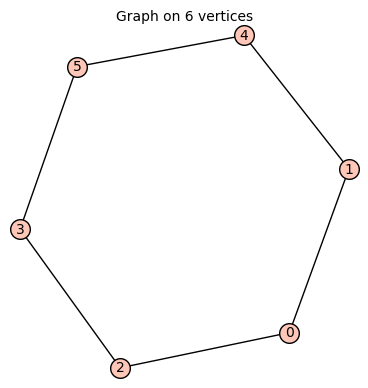
\includegraphics[width=5cm, height=5cm]{MAX_6}
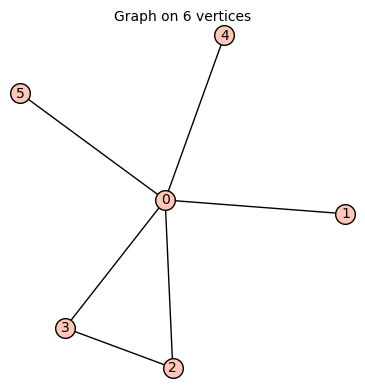
\includegraphics[width=5cm, height=5cm]{MIN_6} \\
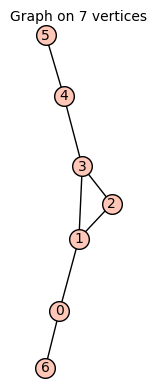
\includegraphics[width=2cm, height=5cm]{MAX_7}
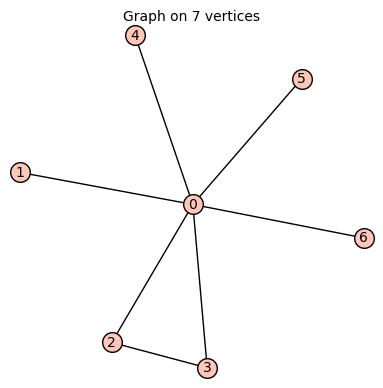
\includegraphics[width=5cm, height=5cm]{MIN_7} \\
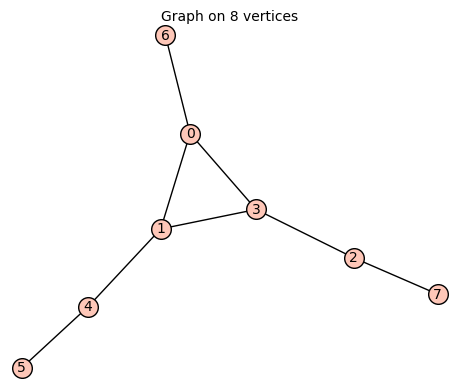
\includegraphics[width=5cm, height=5cm]{MAX_8}
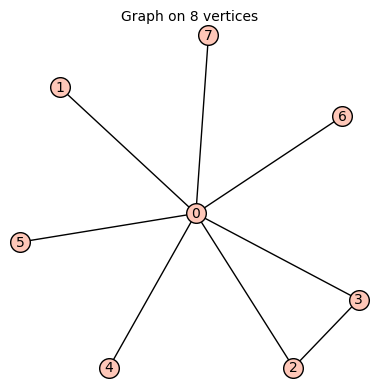
\includegraphics[width=5cm, height=5cm]{MIN_8} 
\end{center}

Za drugi del naloge, smo pri majhnih drevesih ugotovili, da je minimalna $\textit{AZI}_{\alpha}$ vrednost pri $\alpha > 0$, zvezdaste oblike. Zanimivo je, da pri $-\alpha$ ti grafi dosežejo maksimalne vrednosti.  Zdi se nam, da ta opazka pri večanju števila vozlišč $n$ ne bo veljala. 

\begin{center}
Maksimalni grafi \\
$\alpha = -3$ \quad  \quad \quad \quad \quad \quad \quad \quad \quad \quad \quad $\alpha = 3$ \quad\\
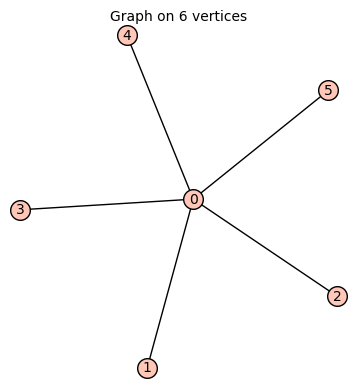
\includegraphics[width=5cm, height=4cm]{AZI_alpha/max_n6_a-3}
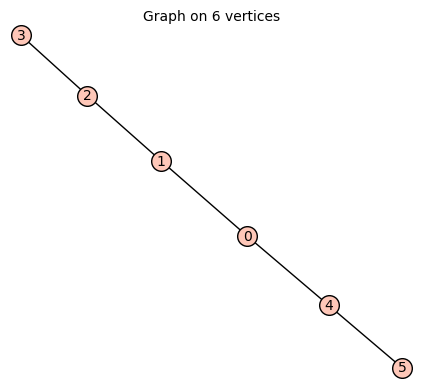
\includegraphics[width=5cm, height=4cm]{AZI_alpha/max_n6_a3}\\
\pagebreak
Minimalni grafi \\
$\alpha = -3$ \quad  \quad \quad \quad \quad \quad \quad \quad \quad \quad \quad $\alpha = 3$ \quad\\
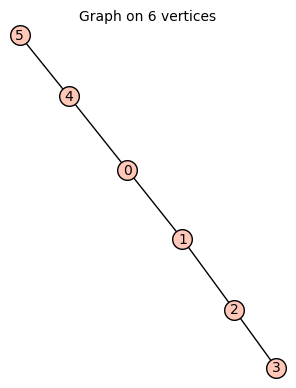
\includegraphics[width=5cm, height=4cm]{AZI_alpha/min_n6_a-3}
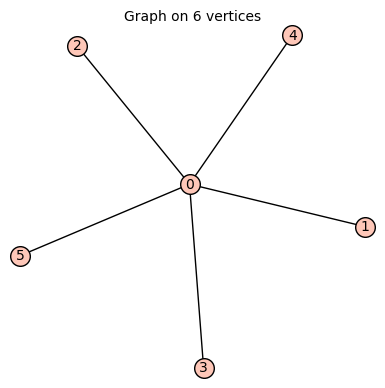
\includegraphics[width=5cm, height=4cm]{AZI_alpha/min_n6_a3}


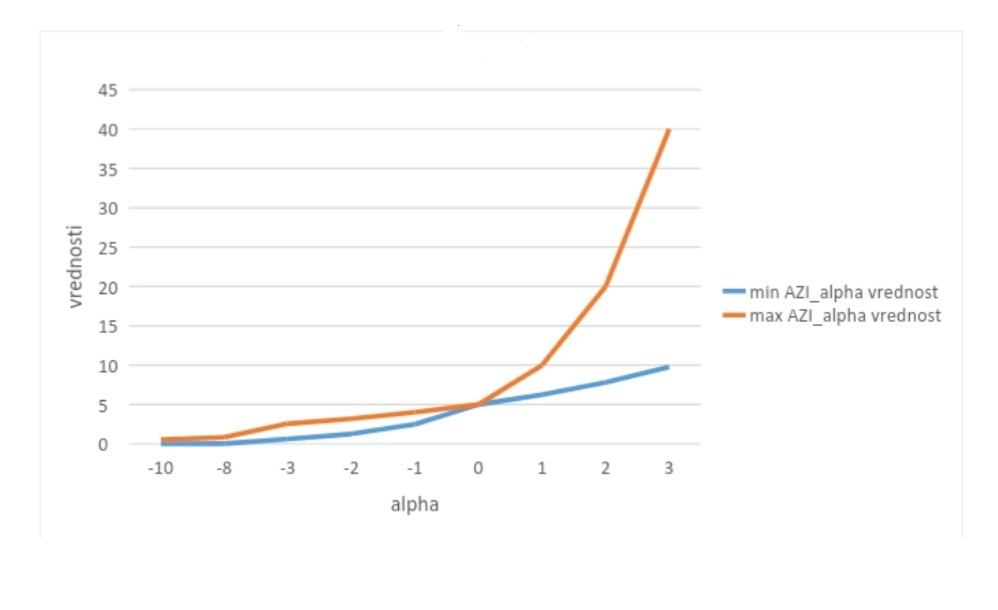
\includegraphics[width=13cm]{AZI_alpha/n=6}
\end{center}

Iz zgornjega grafa je razvidno, da minimalna in maksimalna $AZI$ vrednost v odvisnosti od $\alpha$ strogo naraščata in se dotikata v $\alpha = 0$ 


\section{Analiza z uporabo algoritmoma Simulating Annealing}
Pri iskanju ekstremnih vrednosti na grafih z več kot 8 vozlišči smo uporabili \textit{Simulating Annealing} algoritem. Najprej s pomočjo vgrajenih fukcij generiramo začetni graf, ki ustreza našim kriterijem ( v prvem delu naloge mora veljati, da je graf enocikličen, v drugem pa mora biti graf drevo) na tem začetnem grafu pa poženemo naš algoritem. Algoritem deluje v dveh korakih:
\begin{itemize}
\item{spreminjanje trenutnega grafa}
\item{primerjanje $AZI$ vrednosti trenutnega in do sedaj najboljšega grafa}
\end{itemize}
Pri tem moramo poudariti, da spreminjanje trenutnega grafa poteka tako, da trenutnemu grafu odvzamemo eno povezavo. Nato želim naključno dodati novo povezavo vendar moramo pri tem zadostiti pogoju enocikličnosti. Zato preverimo katero od povezav smo od grafa odstarnili. Če je bila odvzeta povezava drevesna moramo novo dodati tako, da ponovno povežemo obe komponenti. Če pa graf ostane povezan moramo novo povezavo dodati na način, da ustvarimo cikel. V našem primeru bo katera koli nova povezava temu zadostila.\\
Za drugu del naloge poganjamo algoritem na drevesih zato je pri generiranju trenutnega grafa tako ali tako možna samo prva varianta. 

\subsection{Psevdokoda}

Koda za generiranje naključnega (enocikličnega) grafa.
\begin{lstlisting}
def generiranje_grafa(n):
    A = graphs.RandomTree(n)
    A.add_edge(A.complement().random_edge(labels=False))
    return A
\end{lstlisting}

\textbf{\textit{Simulating Annealling} algoritem.}
\begin{lstlisting}
from random import choice
def maxima(graf, n=100000, alpha=3):
    i = 0
    najboljsa = trenutna = AZIvrednost(graf, alpha)
    najboljsi_graf = graf
    for j in range(n):
        T = n/(j+1)
        e = graf.random_edge(labels=False)
        i += 1
        K = Graph(graf)
        if i > n:
            return(AZIvrednost(K, alpha))
        K.delete_edge(e)
        if K.is_connected():
            e = K.complement().random_edge()
        else:
            A, B = K.connected_components()
            e = (choice(A), choice(B))
        K.add_edge(e)
        a = AZIvrednost(K, alpha)
        if a > najboljsa:
            najboljsi_graf = K
            najboljsa = a
        if a > trenutna or exp((trenutna - a) / T) > random():
            graf = K
            trenutna = a
    najboljsi_graf.show()
    return (najboljsi_graf, najboljsa)
\end{lstlisting} 

\subsection{Rezultati}

Pri analizi $AZI$ vrednosti na enocikličnih grafih ugotovimo, da se z večanjem števila vozlišč hipoteza o obliki zvezde grafa z minimalno vrednostjo ne uresniči v celoti. Morda je krivo tudi dejstvo, da za večje grafe izvedemo premalo korakov (mi smo jih izvedli za vsak algoritem okoli 100.000). Morda bi ob večjem številu ponovitev grafi na koncu le prišli zvezdaste oblike. Ne glede na to pa je razvidno, da imajo grafi, ki dosežejo minimalno vrednost, obliko (nekaj) povezanih zvezd. Za grafe z maksimalnimi vrednostmi drži načelo zmanjševanja števila listov vendar ne popolnoma, saj bi v nasprotnem tvorili en sam velik cikel (primer tega je podan že pri $n=8$). 

\begin{center}
\textbf{Maksimalni (levi) in minimalni (desni) grafi} \\
\textbf{$n=10$}\\
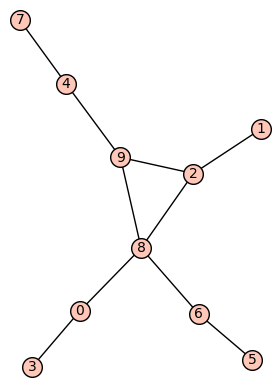
\includegraphics[width=5cm, height=5cm]{MAX_10}
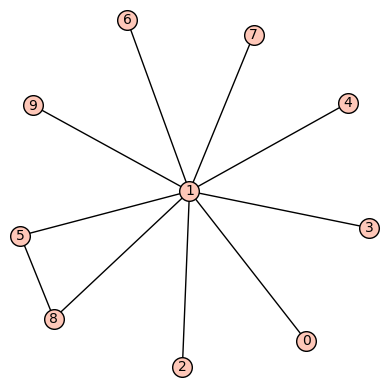
\includegraphics[width=5cm, height=5cm]{MIN_10} \\
\textbf{$n=50$}\\
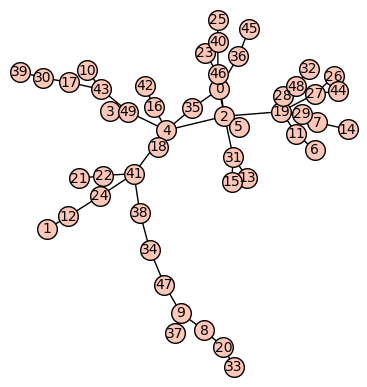
\includegraphics[width=7cm, height=7cm]{MAX_50}
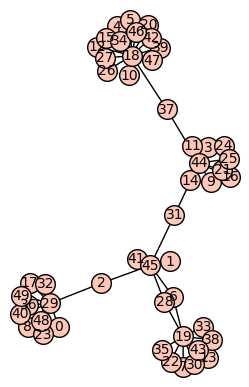
\includegraphics[width=7cm, height=7cm]{MIN_50} \\
\pagebreak
\textbf{$n=100$}\\
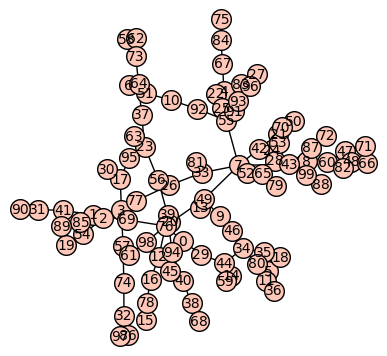
\includegraphics[width=7cm, height=7cm]{MAX_100}
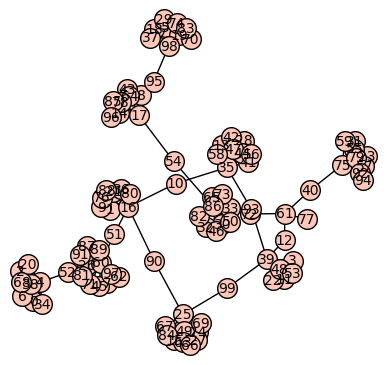
\includegraphics[width=7cm, height=7cm]{MIN_100} 
\end{center}

Na drevesih pri več vozliščih moram ovreči zgornjo hipotezo o usklajenosti dreves glede na predznak $\alpha$. Pri maksimalni vrednosti za $\alpha$ in minimalni vrednosti za $-\alpha$ se grafa torej ne ujemata. Morda bi se grafi po več korakih manj razlikovali vendar dvomimo, da bi prišli identični. Tako kot pri enocikličnih grafih se zvezdasta oblika za dano število korakov ne ohranja pri večanju števila vozlišč. 

\pagebreak
\begin{center}
Maksimalni grafi pri $n=100$\\
$\alpha = -10$ \quad  \quad \quad \quad \quad \quad \quad \quad \quad \quad \quad $\alpha = 10$ \quad\\
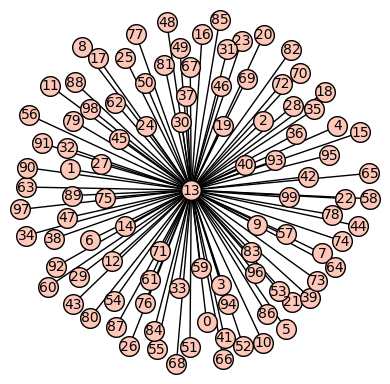
\includegraphics[width=7cm, height=7cm]{AZI_alpha/max_n100_a-10}
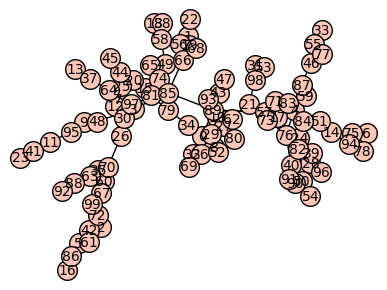
\includegraphics[width=7cm, height=7cm]{AZI_alpha/max_n100_a10}\\
Minimalni grafi pri $n=100$\\
$\alpha = -10$ \quad  \quad \quad \quad \quad \quad \quad \quad \quad \quad \quad $\alpha = 10$ \quad\\
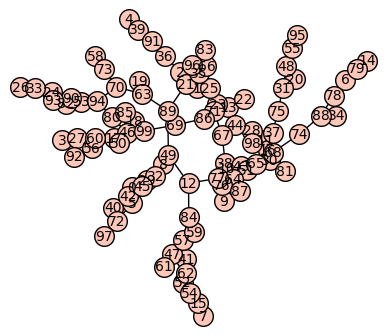
\includegraphics[width=7cm, height=7cm]{AZI_alpha/min_n100_a-10}
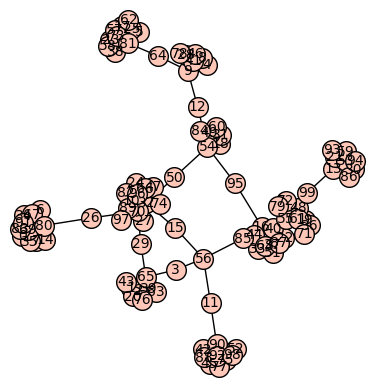
\includegraphics[width=7cm, height=7cm]{AZI_alpha/min_n100_a10}
\end{center}


Iz spodnjih grafov vidimo kako se gibljejo minimalne in maksimalne ${AZI}_{\alpha}$ vrednosti ob povečevanju $\alpha$ ter povečevanju število vozlišč. ${AZI}_{\alpha}$ vrednosti strogo naraščajo, kar je posledica večanja števila vozlišč.

\pagebreak
\begin{center}
Minimalna ${AZI}_{\alpha}$ vrednost\\
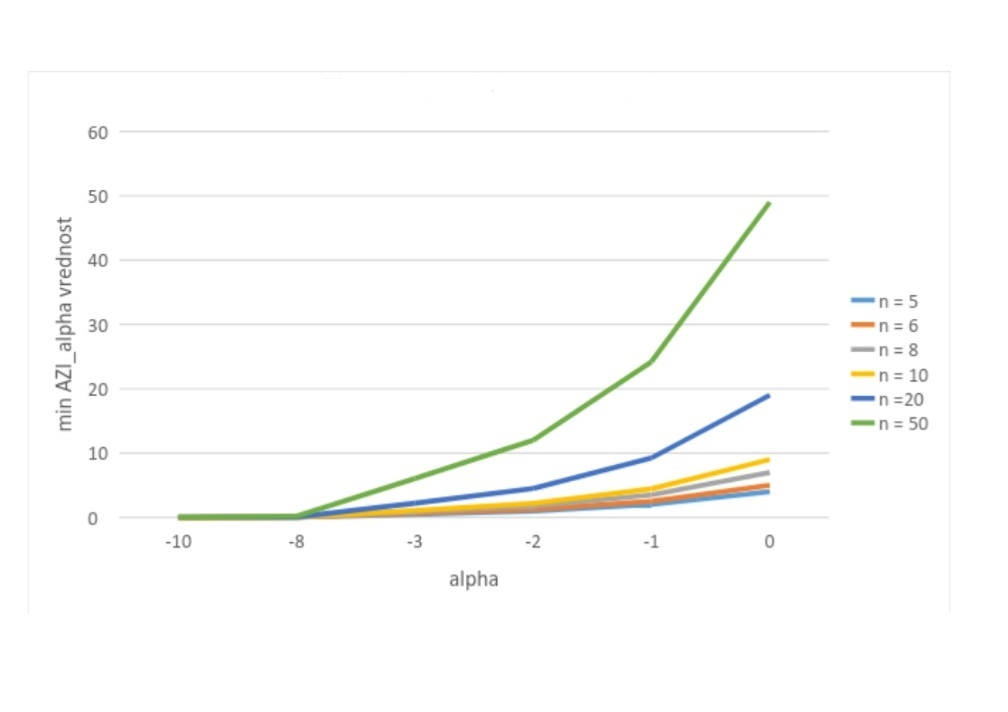
\includegraphics[width=15cm]{AZI_alpha/IMG_20200109_163631}
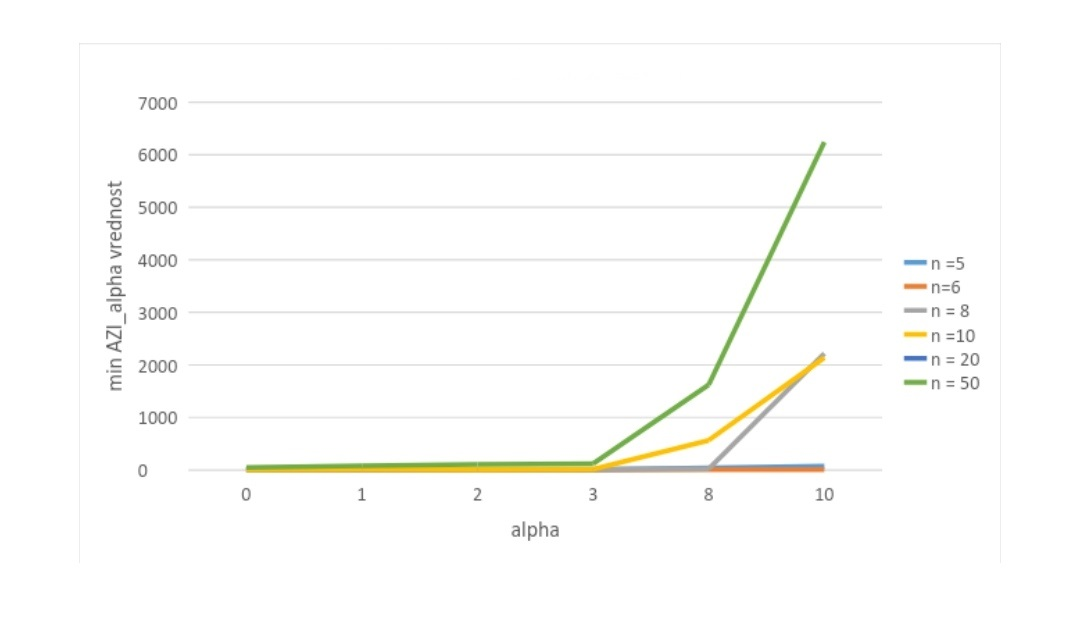
\includegraphics[width=15cm]{AZI_alpha/IMG_20200109_163647}\\
\pagebreak
Maksimalna ${AZI}_{\alpha}$ vrednost\\
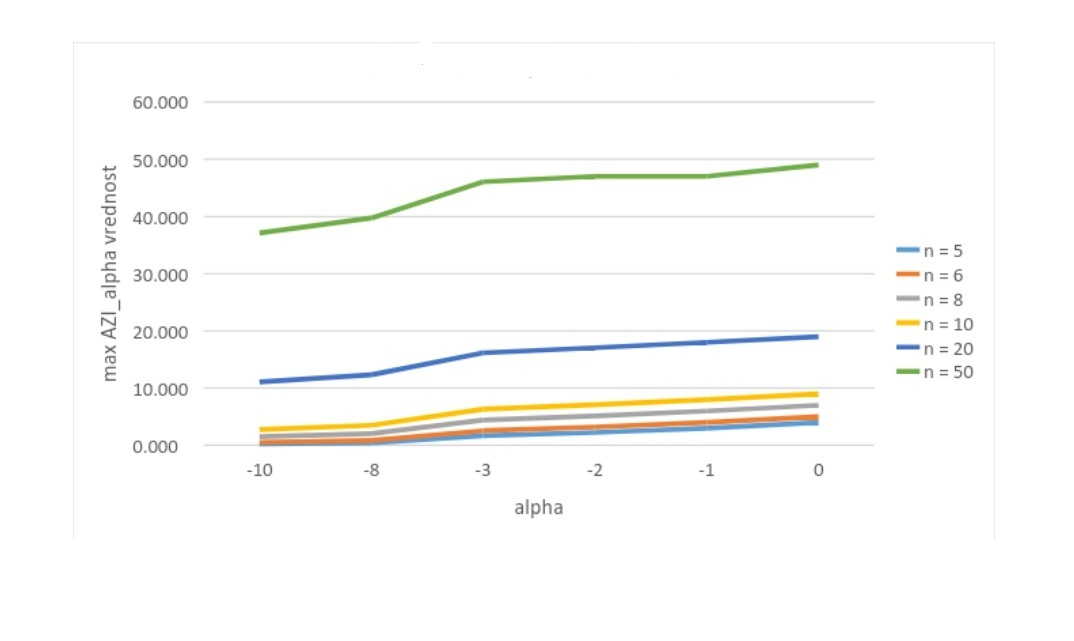
\includegraphics[width=15cm]{AZI_alpha/IMG_20200109_163930}
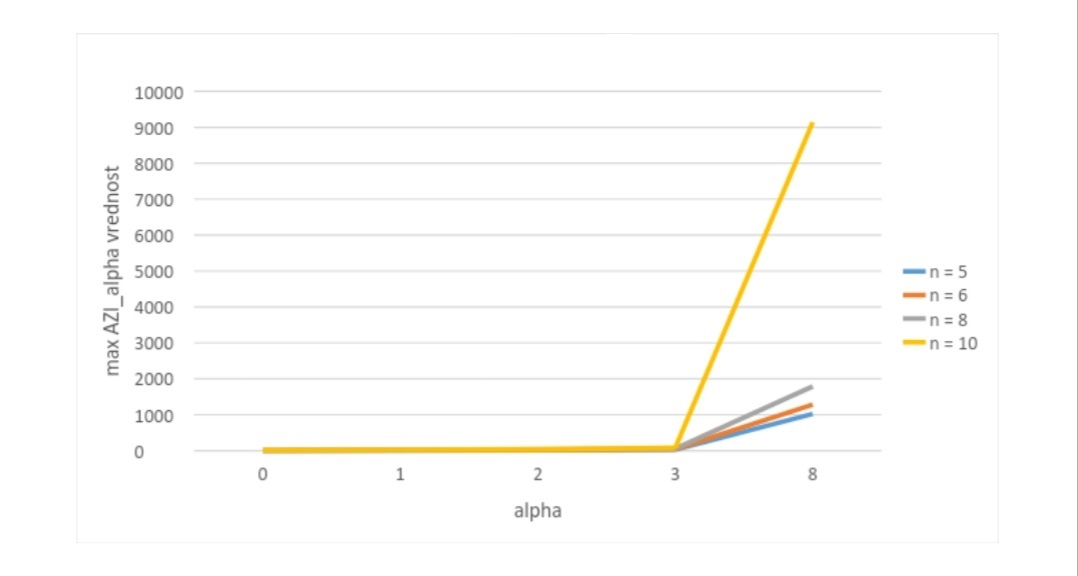
\includegraphics[width=15cm]{AZI_alpha/IMG_20200109_164007}



\end{center}


\end{document}
